\documentclass[aspectratio=1610]{beamer}
\usetheme{Hannover}
\usepackage{graphicx}
\usepackage{wrapfig}
\usepackage{multimedia}
%Title%
\title{Analysing Survey Data in R}
\subtitle{FOAR705 Proof of Concept presentation}
\author{Kathryn Phillips, 43686826} 
\institute{Department of International Studies}
\date{\today}
%document%
\begin{document}
%content goes here%
%Title page%
\begin{frame}
\frame{\titlepage}
\end{frame}
%contents table%
\begin{frame}
\frametitle{Table of Contents}
\tableofcontents
\end{frame}
%section one -Introduction%%%%%%%
\section{Introduction}
\subsection{My Research Topic}
%%%%%%%%%%%%%%%%%%%%%%%%%%%%%%%%%
\begin{frame}
\frametitle{My Research Topic}
During my MRes course, I plan to research the influence of Korean Pop (Kpop) within Japan.
\newline
You can find advertisements for Kpop all around Tokyo, but where is the research on this phenomenon?
\newline
\begin{figure}[h]

\includegraphics[scale=0.2]{bts}
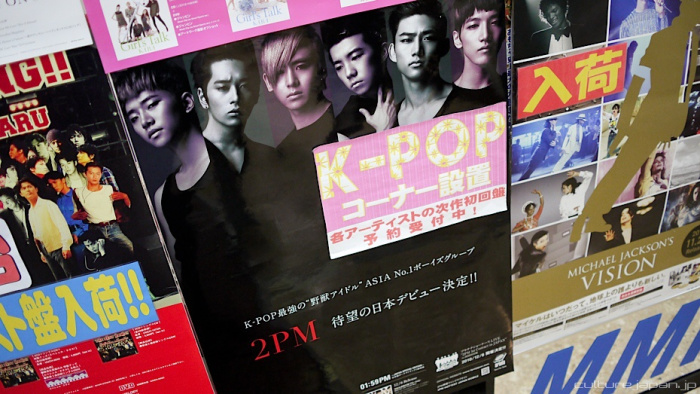
\includegraphics[scale=0.6]{kpopexample}
\end{figure}
\movie[width=2cm,height=2cm,poster]{\em Click here for an example of Kpop}{short.mp3}
\end{frame}
%%%%%%%%%%%%%%%%%%%%%%%%%%%%%%%%%%
\subsection{Data Analysis in R}
%%%%%%%%%%%%%%%%%%%%%%%%%%%%%%%%%%
\begin{frame}
\frametitle{Data Analysis in R}
%include font and spacing?%
I used R to form a code line that could analyse specific groups of responses out of the thousands I could receive from an online survey.
R allows me to:
\begin{itemize}
\item Immediately take online responses from surveys
\item Input them into a well-structured database
\item Select specific groups within the database
\item Create graphs of my data
\end{itemize}
With this tool chain, I am well-prepared to start my research in the months to come!
 \end{frame}
%section 2 - Initial Scoping (subsection - selection)%%%%%%%
\section{Scoping}
\subsection{Selection}
%%%%%%%%%%%%%%%%%%%%%%%%%%%%%%%%%%%
\begin{frame}
\frametitle{Scoping}
\framesubtitle{Selection}
%font and spacing to be added%
Initially, I had several areas where using a digital tool could improve the flow and pace of my work.
\begin{itemize}
\item Compiling sources for literature research
\item Analysis of survey data
\item Transcription and Translation of Interviews
\item Writing and formatting my final Thesis
\end{itemize}
Out of these four areas, I considered survey data analysis to be the most time-consuming, so I decided to work on saving time here through implementing a digital tool.
\end{frame}
%%%%%%%%%%%%%%%%%%%%%%%%%%%%%%%%%%%%%%%
\subsection{Elaboration}
%%%%%%%%%%%%%%%%%%%%%%%%%%%%%%%%%%%%%%%
\begin{frame}
\frametitle{Scoping}
\framesubtitle{Elaboration}
In order to choose the correct tool to use, I had to refine my input and output sources. These went through many iterations, but eventually ended up like this:
\begin{itemize}
\item Input: Raw data collected from an online survey site that is capable of producing both qualitative and quantitative data and presenting it in a spreadsheet (CSV) format.
\item Output: A dataset that can receive queries for specific subsets, answer these queries and plot the results in a graphical format.
\end{itemize}
Due to my choice of input and output, I was able to pick R as my intended tool-of-choice.
\end{frame}
%New Section - Implementation%%%%
\section{Implementation}
\subsection{Creating a Tool Chain}
%%%%%%%%%%%%%%%%%%%%%%%%%%%%%%%%%
\begin{frame}
\frametitle{Implementation}
\framesubtitle{Creating a Tool Chain}
I needed to prove that R could take a basic spreadsheet (CSV) input and create my desired output. To do this, I created my own small table of data, before loading it into the R environment and constructing a plot.  
\newline
\newline
This tool chain was a success, so I was then able to continue onto using more complex data, in a similar style to what I intended on using in my final thesis.
\end{frame}
%%%%%%%%%%%%%%%%%%%%%%%%%%%%%%%%%%%%%%%
\subsection{Elaborating on my Chain}
%%%%%%%%%%%%%%%%%%%%%%%%%%%%%%%%%%%%%%%
\begin{frame}
\frametitle{Implementation}
\framesubtitle{Elaborating on my Chain}
Now I knew that my tool chain worked with simple data, created a more complicated chain. 
\begin{center}
Google Forms survey (real-world data collection) 
\newline
$\,\to\,$
Data analysis in R
\newline
$\,\to\,$ 
Graph imported into a Word document
\end{center}
The survey was completed by my FOAR705 class. With this new data I created a tabular database that could answer all the questions I asked.
\end{frame}
%%%%%%%%%%%%%%%%%%%%%%%%%%%%%%%%%%%%%%
\subsection{The Database}
%%%%%%%%%%%%%%%%%%%%%%%%%%%%%%%%%%%%%%
\begin{frame}
\frametitle{Implementation}
\framesubtitle{The Database}
In order to avoid errors when asking my data various questions, I broke the database down into a number of connected tables.
\newline
\begin{figure}[h]
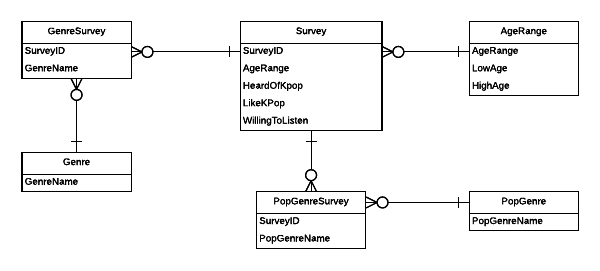
\includegraphics[scale=0.35]{Diagram}
\end{figure}
These could be joined together at will when necessary for answering a question.
In order to prove my concept, I decided to examine 18-29 year olds' music tastes, and place the data into a bar plot.
\end{frame}
%%%%%%%%%%%%%%%%%%%%%%%%%%%%%%%%%%%%%%%
\section{Results}
\subsection{Pros}
%%%%%%%%%%%%%%%%%%%%%%%%%%%%%%%%%%%%%%%
\begin{frame}
\frametitle{Results}
\framesubtitle{Pros:}
\begin{itemize}
\item General growth of my technical skillset
\item Success in using R to create simple tool chains
\item Increased knowledge of technical tools available for implementation in a range of tasks
\item The structure of the database can be used for much larger spreadsheets with thousands of entries
\end{itemize}
\begin{figure}[h]
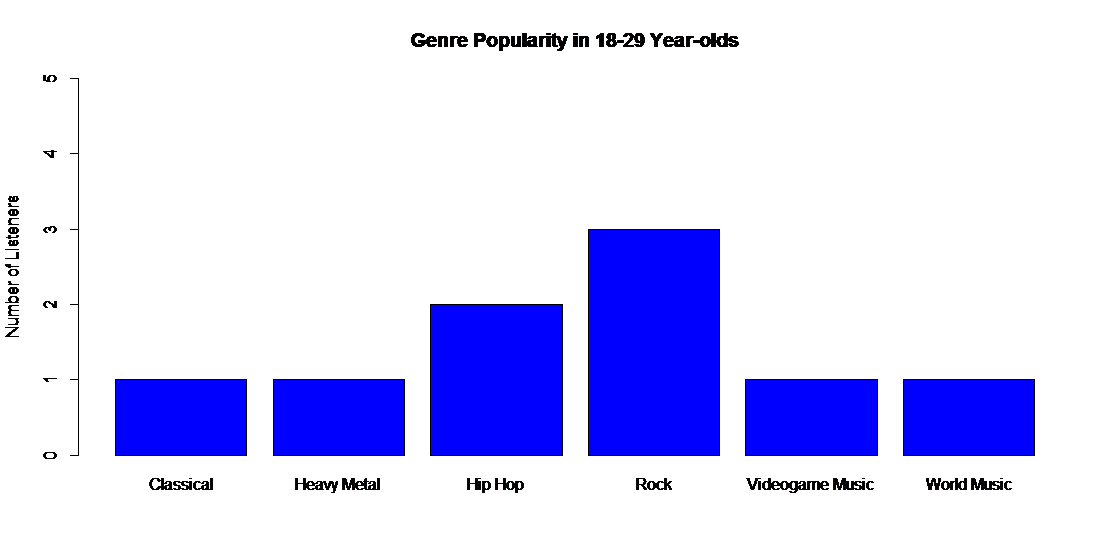
\includegraphics[scale=0.3]{Final}
\end{figure}
\end{frame}
%%%%%%%%%%%%%%%%%%%%%%%%%%%%%%%%%%%%%%%
\subsection{Cons}
%%%%%%%%%%%%%%%%%%%%%%%%%%%%%%%%%%%%%%%
\begin{frame}
\frametitle{Results}
\framesubtitle{Cons:}
\begin{itemize}
\item R support online is often outdated for the current version (code changes)
\item Time is still currently an issue in terms of utilising this tool - however, I would say that if R is implemented properly, there will likely be fewer problems concerning data breaking under manipulation. 
\end{itemize}
\end{frame}
%%%%%%%%%%%%%%%%%%%%%%%%%%%%%%%%%%%%%%%
\section{Conclusion}
\subsection{Final Words}
%%%%%%%%%%%%%%%%%%%%%%%%%%%%%%%%%%%%%%%
\begin{frame}
\frametitle{Conclusion}
My implementation of R as a tool for data analysis has been successful.
\newline 
I am now able to ask questions of R, and receive graphical responses with ease.
\newline 
This success means that I can replicate the same process shown here with my thesis data with minimal difficulty.
\end{frame}
%%%%%%%%%%%%%%%%%%%%%%%%%%%%%%%%%%%%%%%
\subsection{Code Repository}
%%%%%%%%%%%%%%%%%%%%%%%%%%%%%%%%%%%%%%%
\begin{frame}
\frametitle{Conclusion}
\framesubtitle{Code Repository}
If you would like to have a look at my code and the collected data used in this project, please follow the link below:
\newline
\newline
\url{https://github.com/Kattkin/FOAR705-Coding-line}
\end{frame}
 %done!%
\end{document}